\documentclass[letterpaper]{article}

\usepackage{aaai}
\usepackage{times}
\usepackage{helvet}
\usepackage{courier}
\usepackage{hyperref}
\usepackage{tabularx}
\usepackage{siunitx}
\usepackage{graphicx}
\usepackage{todonotes}
\sisetup{output-exponent-marker=\ensuremath{\mathrm{e}}}

\frenchspacing
\setlength{\pdfpagewidth}{8.5in}
\setlength{\pdfpageheight}{11in}
\pdfinfo{
    /Title (Email Autoresponder using a Sequence-to-sequence Architecture with BERT)
    /Author (Claudio Scheer, Jos\'e Fernando Possebon)
}
\setcounter{secnumdepth}{0}
\begin{document}
% The file aaai.sty is the style file for AAAI Press 
% proceedings, working notes, and technical reports.
%
\title{Email Autoresponder using a Sequence-to-sequence\\Architecture with BERT}
\author{Claudio Scheer \and Jos\'e Fernando Possebon\\
    Pontifical Catholic University of Rio Grande do Sul - PUCRS\\
    \{claudio.scheer, jose.possebon\}@edu.pucrs.br
}

\maketitle

\begin{abstract}
    \begin{quote}
        Due to the large number of emails that people receive, it is not just about filtering what is spam or not, but it is also essential to help people filter what requires their attention from something that can be done by an intelligent agent. If we consider the scenario of a sales representative who sells software licenses, for example, it is common to receive requests for quotations from their customers about the price of software licenses. We believe that it is possible to implement an agent that could read the emails, understand what is requested, and respond to their emails automatically.
    \end{quote}
\end{abstract}

\noindent Introduction.


\section{Related works}
Related works.


\section{Deep Learning}

In this section, we will discuss the sequence-to-sequence model using recurrent neural networks and transformers. In addition, we also discuss how a BERT model works.

\subsection{Sequence-to-sequence}

The encoder-decoder architecture was initially proposed by \cite{DBLP:journals/corr/ChoMGBSB14}. Although simple, the idea is powerful: use a recurrent neural network to encode the input data and a recurrent neural network to decode the encoded input into the desirable output. Two neural networks are trained.

\cite{DBLP:journals/corr/Graves13} - Generating sequences with LSTM

- Attention is all you need


\subsection{BERT}

BERT is a short for Bidirectional Encoder Representations from Transformers, proposed by \cite{DBLP:journals/corr/abs-1810-04805}. Transformers network was proposed by \cite{DBLP:journals/corr/VaswaniSPUJGKP17} and use the attentions mechanism, proposed by \cite{DBLP:journals/corr/BahdanauCB14}, to learn representations between words that can express their contextual meaning.

The original BERT model was pre-trained in a corpus comprising Wikipedia and Book Corpus. BERT has two pre-trained models available: BERT large, with \num{345}{M} parameters (24 layers) and BERT base, with \num{110}{M} (12 layers).

The model was pre-trained for masked language modeling nas next sentence predictions tasks. However, with the replacement of the last layer and fine-tuning, the model can be used for other tasks, using the same parameters as the original BERT model.


discuss it here

In a nutshell, the difference is that self-attention is only applied to the input sequence, while cross-attention is applied to the input and output sentences.


\section{Dataset}

As the project focus is on automatic email reply, The Enron Email Dataset\footnote{\href{https://www.kaggle.com/wcukierski/enron-email-dataset}{https://www.kaggle.com/wcukierski/enron-email-dataset}} was used to train the model. The dataset contains only the emails raw data. Therefore, a parser\footnote{\href{https://www.kaggle.com/claudioscheer/extract-reply-emails}{https://www.kaggle.com/claudioscheer/extract-reply-emails}} was built to extract the email and the replies from the raw data of the email.

To identify whether an email has a reply or not, we look for emails that contain the string \texttt{-----Original Message-----}. After filtering only emails with non-empty replies, those emails were parsed into an input sequence (the original email) and a target sequence (the reply email). The entire extraction was done automatically, that is, we did not extract or adjust any email manually.

Two libraries were used to parse the dataset: \texttt{talon}\footnote{\href{https://github.com/mailgun/talon}{https://github.com/mailgun/talon}}, provided by Mailgun, and \texttt{email}, provided by Python. The \texttt{email} package returns the email body with the entire thread. To extract only the last reply from an email thread, the \texttt{talon} package was used.

The original dataset contains \num{517401} raw emails. After parsing the raw dataset, the new dataset consisted of \num{110205} input and target pairs. As the resources available to fine-tune the model were limited,  only emails with less than \num{256} characters were used. The final dataset consisted of \num{40062} emails. All of these input and target pairs were used to train the BERT model.

\num{21} emails that were not correctly parsed were used to evaluate the model and obtaing the BLEU score. These emails were chosen manually from the dataset.


\section{Implementation}

A pre-trained BERT model, provided by Hugging Face\footnote{\href{https://huggingface.co/}{https://huggingface.co/}}, was used. Hugging Face also provides a PyTorch library for using the pre-trained models. Therefore, this library was used to implement the sequence-to-sequence model, with PyTorch 1.5.1.

The \texttt{BertModel} class provided by Hugging Face can behave as an encoder or decoder. The difference is that, for the encoder, only a layer of self-attention is used and, for decoder, a layer of cross-attention is added between the layers of self-attention. The difference between these attention mechanisms is discussed in Section~BERT.

In this paper, the BERT base architecture was used. This model uses fewer resources, which allowed us to increase the batch size. To fine-tune the model, the following hyperparameters was used:

\begin{itemize}
    \item Learning rate: \num{1e-4};
    \item Warm-up steps: \num{5000};
    \item Epochs: \num{10.5};
    \item Adam epsilon: \num{1e-4}, same as in the original BERT paper \cite{DBLP:journals/corr/abs-1810-04805};
    \item Batch size: \num{10};
    \item Beam search hypothesis: \num{3};
\end{itemize}

In the fine-tune process, an EC2 spot instance on AWS was used. A checkpoint of the model was saved every \num{20000} steps, mitigating the loss of processment if the instance was suddenly stopped. The instance was equipped with a 16 GB NVIDIA T4 GPU (CUDA 10.2).

The batch size was limited by the amount of GPU memory available. We also tested to accumulate and update the gradients after \num{4} steps, but we did not see any improvements.

Different values were tested for the learning rate and epochs, with and without warm-up. Figure~\ref{fig:learning-rate-schedule} shows the final results of the learning rate update during the fine-tuning process.

\begin{figure}[ht]
    \centering
    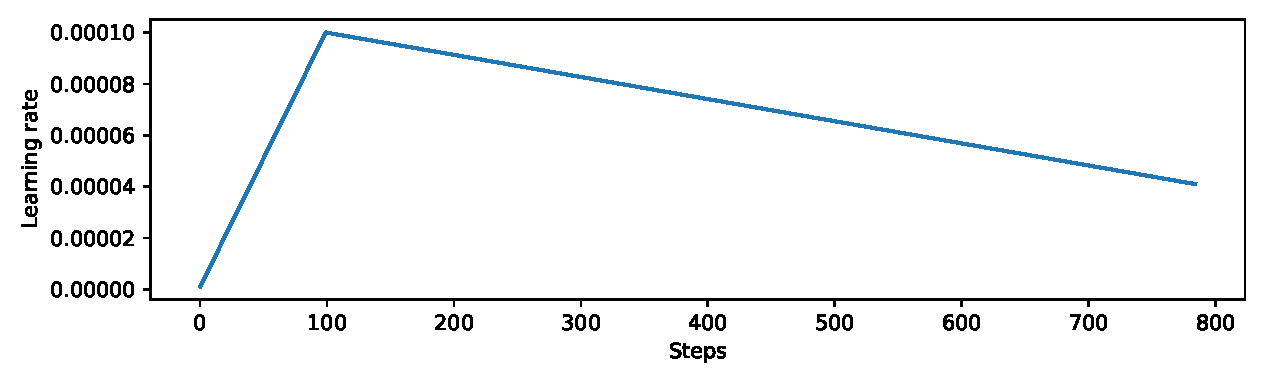
\includegraphics[width=0.47\textwidth]{../images/warmup_linear_schedule.pdf}
    \caption{Learning rate schedule}
    \label{fig:learning-rate-schedule}
\end{figure}

Figure~\ref{fig:loss} shows the loss function value over the fine-tuning process. We do not know why, but loss function shows a greater decrease at the end of each epoch.

\begin{figure}[ht]
    \centering
    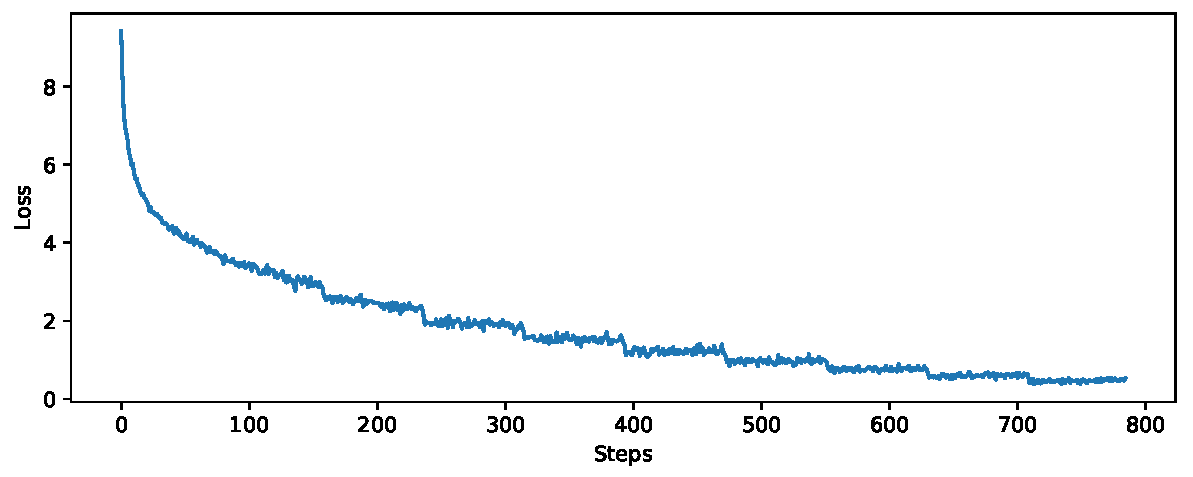
\includegraphics[width=0.47\textwidth]{../images/loss_function.pdf}
    \caption{Loss function}
    \label{fig:loss}
\end{figure}

Some hyperparameters configuration shows bad results in the loss function. For example:

\begin{itemize}
    \item learning rates greater than \num{1e-4} did not make the model converge;
    \item the use of a warm-up period allowed the model to converge in less epochs;
    \item a high number of epochs almost causes an overfitting of the model;
\end{itemize}

The last changed hyperparameter was the number of hypothesis explored in each branch of the beam search. A number greater than \num{3} resulted in more words being out of context in the generated reply email.


\section{Results}

The fine-tuned model still has some noise in the replies generated. Therefore, only the first part of the text of the generated replies was used. This is valid for the BLEU score and for the subjective evaluation.

The BLEU score was used to get a quantitative result of the model. Using the evaluation dataset, the BLEU score was \num{0.0}. This does not mean that the replies were bad. This means that the generated replies do not match to the replies originally sent. Table~\ref{table:example-reply-bleu} shows some examples of why the BLEU score was \num{0.0}.

\begin{table}[ht]
    \centering
    \begin{tabularx}{0.47\textwidth}{|X|X|X|}
        \hline
        \textbf{Input}                                                  & \textbf{Target}                                          & \textbf{Generated}                                                                                                           \\
        \hline
        nevermind.  are you at work?                                    & yea                                                      & i'm all alone over here...                                                                                                   \\
        \hline
        what re your plans for tomorrow?                                & drop prentice's car off at shop; go to dome              & leaving early tomorrow. leaving early. leaving early. leaving early.                                                         \\
        \hline
        I just refaxed it.  For your information, my total hours is 49. & I noted your hours..I will look for the t/s Thanks Lisa! & Thanks Rick, and let's talk after the holidays about a new game plan... Best regards and happy thanksgiving. Jaime Williams. \\
        \hline
    \end{tabularx}
    \caption{Example of generated replies}
    \label{table:example-reply-bleu}
\end{table}

As shown in Table~\ref{table:example-reply-bleu}, BLEU is not a good option for this problem. Therefore, a subjective assessment of the replies was made. We generated some replies, created a form using Google Forms, and asked some people to answer the questionnaire.

The question asked for each reply generated was: Was this reply generated using Artificial Intelligence software? The interviewee could choose only yes or no.

The form contains only five emails and replies. The Table~\ref{table:is-it-ai-test} shows the results of the test answered XXX times. The column AI? shows the percentage of answers that believed the reply was generated by an AI system. The column Correct? shows whether what people believed was correct or not.

\begin{table*}[ht]
    \centering
    \begin{tabularx}{\textwidth}{|X|X|c|c|}
        \hline
        \textbf{Email}                                                                                                                                                                                        & \textbf{Reply}                                                                                                                                                                                                                     & \textbf{AI?} & \textbf{Correct?} \\
        \hline
        Let me know if this works.                                                                                                                                                                            & This works great. Will let you know. as soon as I get a chance, let me know                                                                                                                                                        & \num{0}{\%}  & yes               \\
        \hline
        Following are the terms under which I ran the Forward Obligation report and received this message: General SQL error. ORA-00907: missing right parenthesis. Terms: Let me know what you find. Thanks! & Kate, I ran the report with the exact same options and it came right up. Try it again, exactly as before. Usually if it works for one person and not the other it is a security issue. Let me know what happens. Thanks, Brettther & \num{0}{\%}  & yes               \\
        \hline
        Didn't you trade uranium at one time?                                                                                                                                                                 & Yeah, I know the buisness VERY well.                                                                                                                                                                                               & \num{0}{\%}  & no                \\
        \hline
        Are you free for drinks either Monday or Wednesday?                                                                                                                                                   & Yes                                                                                                                                                                                                                                & \num{0}{\%}  & no                \\
        \hline
        Mons, I would be available on the 25th, 26th or 27th. I cannot make it the week of the 18th. Thanks, Bill.                                                                                            & OK, so, let's see if we can get together later today. I have to leave at 16:00 for a few minutes, but I am sure that I will be out at that moment. Thank you Kim.                                                                  & \num{0}{\%}  & yes               \\
        \hline
    \end{tabularx}
    \caption{Is it AI? test}
    \label{table:is-it-ai-test}
\end{table*}

\todo[inline]{Explain here the results of the form.}


\section{Conclusion}

Despite the small dataset used and limited resources available, the fine-tuned model performed well. In a further works, the dataset must be revised to avoid data that may cause noise in the predictions.



\bibliographystyle{aaai}
\bibliography{references}

\end{document}